\documentclass[nobib]{tufte-handout}

%\\geometry{showframe}% for debugging purposes -- displays the margins

\newcommand{\bra}[1]{\left(#1\right)}
\usepackage{amssymb}
\usepackage{hyperref}
\usepackage[activate={true,nocompatibility},final,tracking=true,kerning=true,spacing=true,factor=1100,stretch=10,shrink=10]{microtype}
\usepackage{color}

% Fixes captions and images being cut off
\usepackage{marginfix}
\usepackage{array}
\usepackage{tikz}
\usepackage{amsmath,amsthm}
\usetikzlibrary{shapes}
\usetikzlibrary{positioning}
\usepackage{listings}
\usepackage{caption}
\DeclareCaptionFont{white}{\color{white}}
\DeclareCaptionFormat{listing}{\colorbox{gray}{\parbox{\textwidth}{#1#2#3}}}
\captionsetup[lstlisting]{format=listing,labelfont=white,textfont=white}

% Set up the images/graphics package
\usepackage{graphicx}
\setkeys{Gin}{width=\linewidth,totalheight=\textheight,keepaspectratio}
\graphicspath{{.}}

\title{Notes for ECE 29595PD - Principles of Digital System Design}
\author[Shubham Saluja Kumar Agarwal]{Shubham Saluja Kumar Agarwal}
\date{\today}  % if the \date{} command is left out, the current date will be used

% The following package makes prettier tables.  We're all about the bling!
\usepackage{booktabs}

% The units package provides nice, non-stacked fractions and better spacing
% for units.
\usepackage{units}

% The fancyvrb package lets us customize the formatting of verbatim
% environments.  We use a slightly smaller font.
\usepackage{fancyvrb}
\fvset{fontsize=\normalsize}

% Small sections of multiple columns
\usepackage{multicol}

% For finite state machines 
\usetikzlibrary{automata} % Import library for drawing automata
\usetikzlibrary{positioning} % ...positioning nodes
\usetikzlibrary{arrows} % ...customizing arrows
\tikzset{node distance=2.5cm, % Minimum distance between two nodes. Change if necessary.
    every state/.style={ % Sets the properties for each state
    semithick,
    fill=gray!10},
    initial text={}, % No label on start arrow
    double distance=2pt, % Adjust appearance of accept states
    every edge/.style={ % Sets the properties for each transition
    draw,
    ->,>=stealth', % Makes edges directed with bold arrowheads
    auto,
    semithick}}
\let\epsilon\varepsilon

% These commands are used to pretty-print LaTeX commands
\newcommand{\doccmd}[1]{\texttt{\textbackslash#1}}% command name -- adds backslash automatically
\newcommand{\docopt}[1]{\ensuremath{\langle}\textrm{\textit{#1}}\ensuremath{\rangle}}% optional command argument
\newcommand{\docarg}[1]{\textrm{\textit{#1}}}% (required) command argument
\newenvironment{docspec}{\begin{quote}\noindent}{\end{quote}}% command specification environment
\newcommand{\docenv}[1]{\textsf{#1}}% environment name
\newcommand{\docpkg}[1]{\texttt{#1}}% package name
\newcommand{\doccls}[1]{\texttt{#1}}% document class name
\newcommand{\docclsopt}[1]{\texttt{#1}}% document class option name

% Define a custom command for definitions and biconditional
\newcommand{\defn}[2]{\noindent\textbf{#1}:\ #2}
\let\biconditional\leftrightarrow

\begin{document}

\maketitle

\begin{abstract}
    These are lecture notes for spring 2024 ECE 29595PD at Purdue. Modify, use, and distribute as you please.
\end{abstract}

\tableofcontents

\section{Course Introduction}

This course serves as an introduction to digital system design, with an
emphasis on principles of digital hardware and embedded system design. It is an
alternate class to ECE 27000. \\ Learning Outcomes:
\begin{enumerate}
    \item Ability to analyze and design combinational logic circuits.
    \item Ability to analyze and design sequential logic circuits.
    \item Ability to analyze and design computer logic circuits.
    \item Ability to realize, test, and debug practical digital circuits.
\end{enumerate}

\pagebreak

\section{Introduction}

Digital design entails creating hardware that can conduct an operation or set
of operations within a computer system. For example, adding two numbers. \\
\begin{center}
    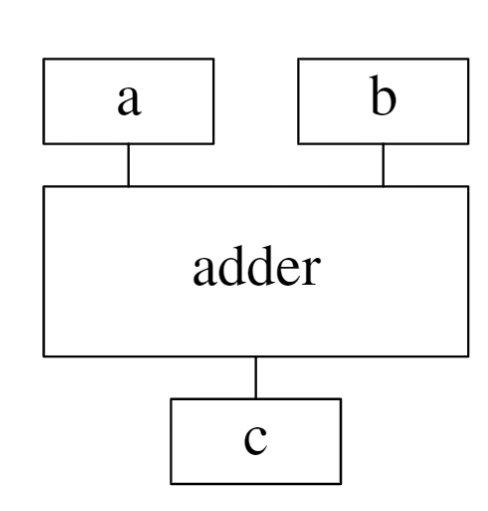
\includegraphics[width= 100px]{images/Screenshot 2024-01-08 151414.png}
\end{center}
This hardware can add two numbers, that is, conduct the operation $c=a+b$. It could also perform $f=d+e$ or $i=g-h=g+(-h)$ as it is not restricted to the sole values of $a$ and $b$ as inputs. This process fits into the logic design and switching algebra portions of chip manufacturing.\\
The creation of systems like these is based on the fact that voltage and current are time-varying and can assume any value in a continuous range of real numbers, but are mapped to only two values.

\subsection{Digital Logic Signals}
A digital signal is modeled assuming that at anytime, it can have only one of
two discrete values, which represent:\\
\begin{table}
    \centering
    \begin{tabular}{c|c}
        0     & 1    \\
        LOW   & HIGH \\
        FALSE & TRUE \\
    \end{tabular}
\end{table}
This is called positive logic.
It maps the infinite values of voltage and current to these two values.
An example of this is CMOS 2-Volt logic:\\
\begin{table}
    \centering
    \begin{tabular}{c|c}
        0      & 1        \\
        \hline
        0-0.5V & 1.5-2.0V \\
    \end{tabular}
\end{table}
These completely separated ranges of values allow for 0 and 1 to be completely separate, with noise and other possible errors being ignored. In this way, all physical values can be partitioned into the two values, though, for intents and purposes of digital system design, voltage is the most relevant.\\
Additionally, circuits known as buffer circuits can be used to restore logic values. That is, if a voltage is not sufficiently close to the values of 0 or 2 (in the case of the CMOS), they can push these values far closer to the desired values, reducing the possibility of error.\\
Digital circuits have replaced analog circuits becuse they are far easier to design. They can be made using Hardware Description Languages (HDLs), softwares that are similar to programming languages.\\
A logic value is called a binary digit, or bit. A set of $n$ bits, represent $2^n$ values. For example:
\begin{table}
    \centering
    \begin{tabular}{c}
        $b_0$ \\
        \hline
        0     \\
        1     \\
    \end{tabular}
    \quad
    \begin{tabular}{c c}
        $b_0$ & $b_1$ \\
        \hline
        0     & 0     \\
        1     & 0     \\
        0     & 1     \\
        1     & 1
    \end{tabular}
\end{table}
\subsection{Logic Circuits}
At the highest level, a logic circuit is a \textit{black box} with $n$ inputs
and $m$ outputs. Only zeros and ones are required to represent inputs and
outputs. \\ Combinational circuits are circuits that have outputs that solely
depend on the inputs. It can be represented by a truth table.\\ An adder can be
represented by a truth table in this manner.
\begin{center}
    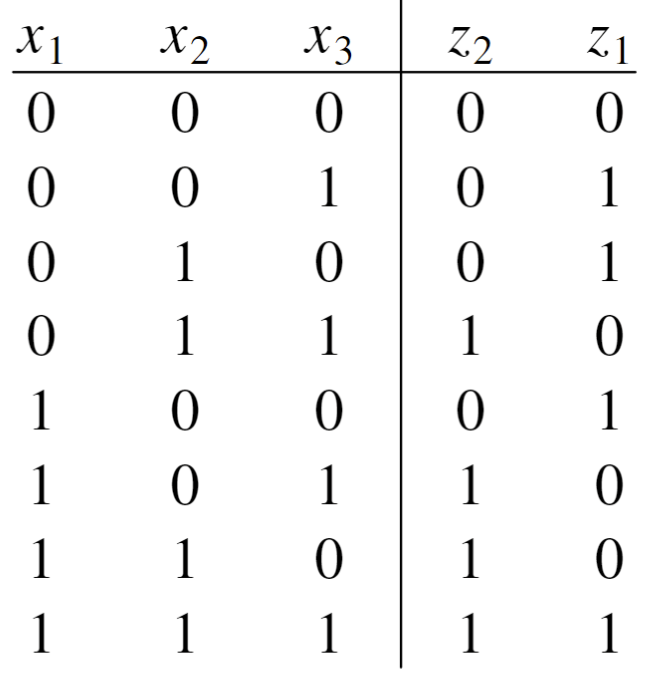
\includegraphics[width= 100px]{images/Screenshot 2024-01-10 144557.png}
\end{center}
On the other hand, a sequential circuit has memory. That is, the output is dependent on both the inputs and the current state of the circuit itself. This is representable through a state table.\\
\begin{center}
    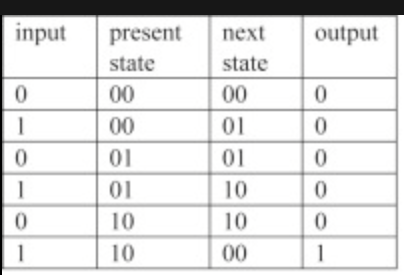
\includegraphics[width= 150px]{images/state table.png}
\end{center}
\subsection{Gates}
Basic digital devices are called gates. These implement basic logic functions.
These are AND, OR, NOT. However, AND, NOT and OR, NOT are sufficient to make
any combination, as the third gate can be formed as a combination of the other
two.\\ Each of the gates is represented symbolically like the following, and
have their truth tables shown below:\\
\begin{table}
    \centering
    \begin{tabular}{c|c|c}
        AND                                                & OR                                                & NOT                                                \\
        \hline
        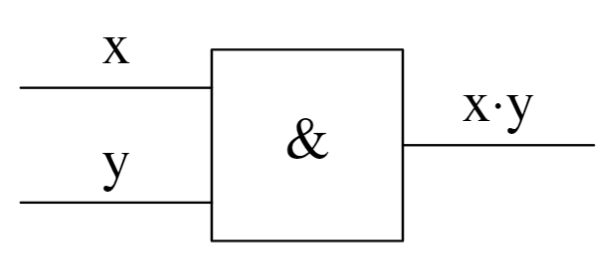
\includegraphics[width= 80px]{images/AND_GATE.png} & 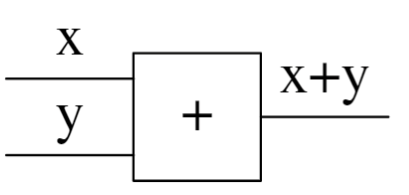
\includegraphics[width= 80px]{images/OR_GATE.png} & 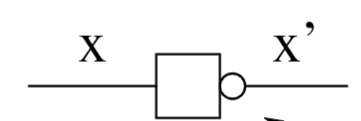
\includegraphics[width= 80px]{images/INVERTER.png} \\
        \hline
        \begin{tabular}{c c|c}
            x & y & {$x\land y$} \\
            \hline
            0 & 0 & 0            \\
            0 & 1 & 0            \\
            1 & 0 & 0            \\
            1 & 1 & 1
        \end{tabular}                            &
        \begin{tabular}{c c|c}
            x & y & {$x\lor y$} \\
            \hline
            0 & 0 & 0           \\
            0 & 1 & 1           \\
            1 & 0 & 1           \\
            1 & 1 & 1
        \end{tabular}                             &
        \begin{tabular}{c|c}
            x & {$\lnot x$} \\
            \hline
            0 & 1           \\
            1 & 0           \\
        \end{tabular}
    \end{tabular}
\end{table}
This can be done for more inputs, by combining multiple gates.\\ There are two more often used gates that can be created through a combination of these two.\\
\begin{table}
    \centering
    \begin{tabular}{c|c}
        NAND                                                & NOR                                                \\
        \hline
        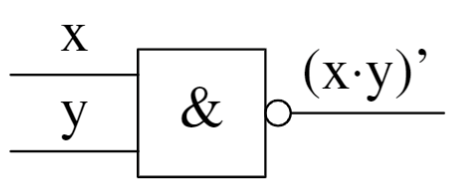
\includegraphics[width= 80px]{images/NAND_GATE.png} & 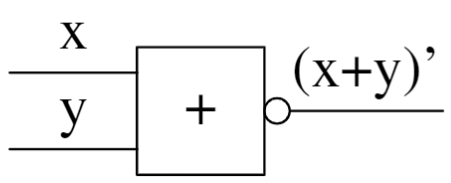
\includegraphics[width= 80px]{images/NOR_GATE.png} \\
        \hline
        \begin{tabular}{c c|c}
            x & y & {$\lnot(x\land y)$} \\
            \hline
            0 & 0 & 1                   \\
            0 & 1 & 1                   \\
            1 & 0 & 1                   \\
            1 & 1 & 0
        \end{tabular}                &
        \begin{tabular}{c c|c}
            x & y & {$\lnot(x\lor y)$} \\
            \hline
            0 & 0 & 1                  \\
            0 & 1 & 0                  \\
            1 & 0 & 0                  \\
            1 & 1 & 0
        \end{tabular}
    \end{tabular}
\end{table}
It is a good exercise to see how two of the basic gates (AND, NOT or OR, NOT) can be used to create the rest, as it is possible to connect gates to form complex circuits and thus, complex functions.\\
\textit{Note: By convention, signal flows from left to right. Thus, output comes out the right and input goes in at left.}
\subsection{Timing}
When the values of an input changes, it takes time for the outputs to change as
well, which is known as \textit{propagation delay}, which can be represented in
a timing diagram. However, for most cases, it is possible ot ignore these, as
the behavior is well defined regardless of delay.\\ The following is a timing
diagram:\\
\begin{center}
    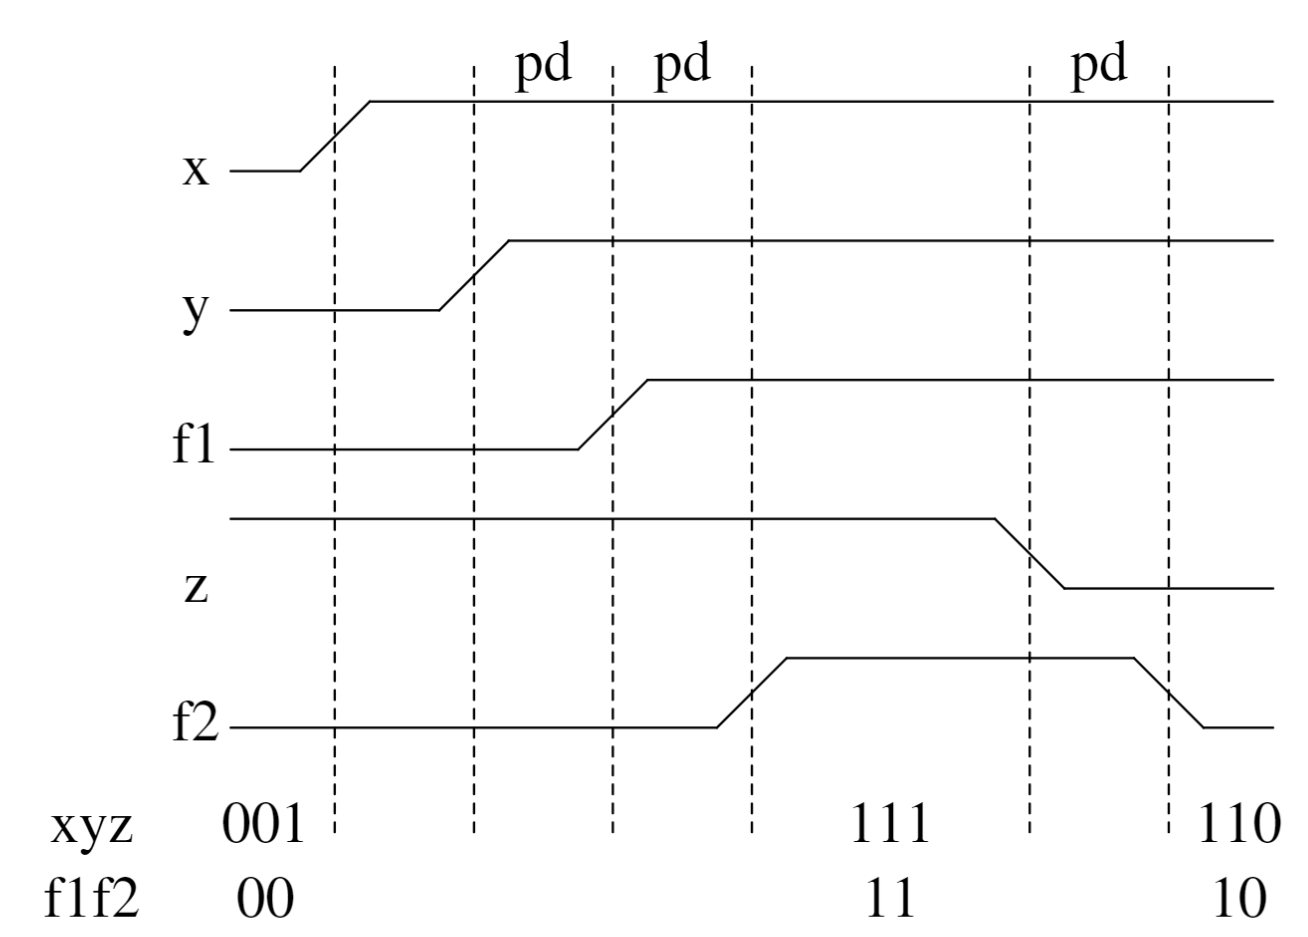
\includegraphics[width= 200px]{images/timing_table.png}
\end{center}
Propagation delay, represented by pd in the timing diagram, is irrelevant if there are no changes, regardless of the fact that there is a new set of inputs. The values at the bottom of the diagram are the values that each of the elements hold after all the necessary transitions have happened for that set of inputs.\\
Transition time is the time it takes for a signal to change from 0 to 1, and is represented by "rt".
\subsection{Software Aspects of Digital Design}
Software is not technically essential to digital system design. People used to
draw symbold by hand, and could make technically equivalent systems. However,
the availability, utility, and ease of use of HDLs has made the use of software
prevalent in the current technological landscape.\\ Electronic Design
Automation tools are useful in improving designer productivity. The following
are examples of these:
\begin{itemize}
    \item Schematic entry: Allows for fully detailed digital diagrams to be created
          digitally.
    \item HDLs: Can be used to design anythong from individual function modules to
          multichip digital systems. This course will involve extensive use of VHDL.
    \item HDL text editors, compilers, synthesizers: text editor to define, compiler to
          debug syntax, synthesizer to create corresponding circuit or chip.
    \item Simulator: It is virtually impossible to debug a synthesized chip, so
          simulators are used before synthesis. They allow for verification of
          functionality prior to the actual tedious process of synthesis. Among
          simulators, there are also PCB simulators, and FPGAs, which are like
          programmable chips. They are very important.
    \item Test benches: Designs are simulated and tested using these. They run a series
          of checks to ensure that nothing stopped working due to changes.
    \item Timing analyzers and verifiers: Correct timing of inputs and reactiosn are
          paramount in digital systems. This facet of simulation allows for the
          automation of timing functionality verification.
    \item Word Processors: Allow for pretty documentation to be created.
\end{itemize}
Software is important, but the understanding of what it actually does is even more so.
\subsection{Integrated Circuits}
A collection of gates on a single silicon chip is called an integrated circuit
or IC.\\ An IC originates from a wafer, which is segmented into many identical
ICs. The wafer is divided into rectangles, called \textit{dies} which in turn
have \textit{pads} which allow for wire connections. Microscopic probes are
used to debug the wafers, and defects are discarded, and the succeses, cut
out.\\ For this class, an IC, is a packaged die.\\ ICs were divided by size,
small SSIs with 1 to 20 gates, medium MSIs with 20 to 200, large LSIs with upto
1000, and vely large VLSIs fro everything above that. The largest VLSIs now
have over 10 billion transistors.\\ An IC process is the steps taken to create
an IC, and are categorized by the transistor density within the chip.
\subsection{Logic Families}
There are many different ways of implementing logic circuits. Connectable logic
circuits are of the same logic family. So, the technology controlling them is
different. Chips need to be from the same family to be connected to each other.
If they are from different families, they cannot be connected to each other.\\
For example TTL (Transistor-Transistor Logic) is a logic family based on
bipolar junction transistors.\\ CMOS (Complementary Metal-Oxide Semiconductor)
is based on MOSFETs (MOS Field-Effect Transistors). These are more commonly
used, and the ones we will be analyzing in this class.\\
\subsection{CMOS Logic Circuits}
A MOS transistor is modellable as a voltage controlled resistor. This means
that the input voltage controls the resistance of the MOSFET, allowing it to
act as a kind of switch. This is because it has only two effective states: very
high resistance and very low resistance.\\ This is an n-channel (NMOS)
transistor:
\begin{center}
    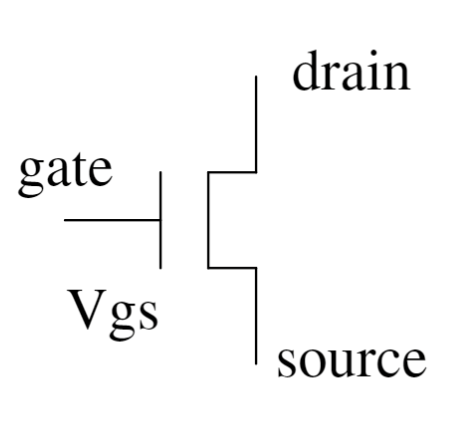
\includegraphics[width= 100px]{images/nmos.png}
\end{center}
When $V_{gs} = 0$, the resistance is very high.\\
When $V_{gs}$ is increased, the resistance is very low.\\
On the other hand, this is the PMOS transistor:\\
\begin{center}
    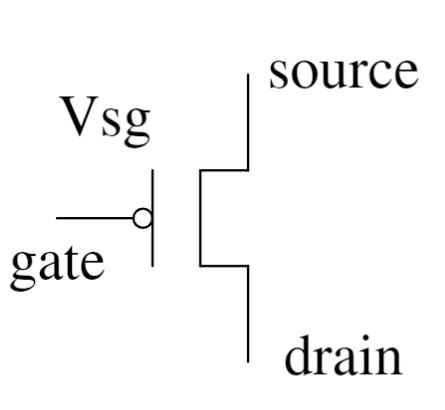
\includegraphics[width= 100px]{images/pmos.png}
\end{center}
When $V_{sg} = 0$, the resistance is very high.\\
When $V_{sg}$ is increased, the resistance is very low.\\
NMOS and PMOS together allow us to form CMOS logic.
For example, this is a CMOS inverter, in which the output will be the opposite of the input.\\
\begin{center}
    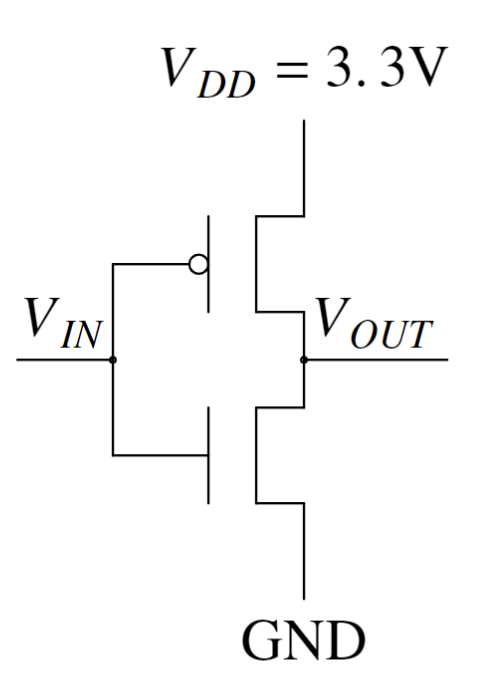
\includegraphics[width= 100px]{images/cmosinverter.png}
\end{center}
If $V_{in} = 3.3V$, or high, the PMOS transistor be off, and the NMOS would be on. This would mean that the output and ground are shorted, causing the output to be low.\\
If $V_{in} = 0V$, or low, the PMOS transistor be on, and the NMOS would be off. This would mean that the output and $V_{DD}$ are shorted, causing the output to be high.\\
This allows this to be act as an inverter.\\
Now we will observe the CMOS arrangement of a NAND gate.
\begin{center}
    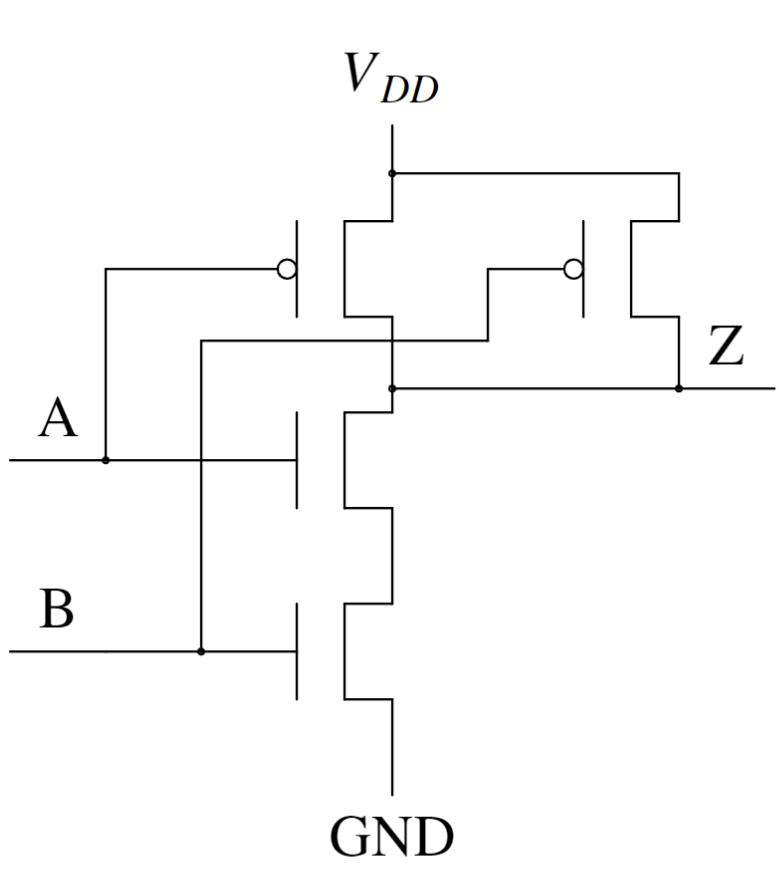
\includegraphics[width= 150px]{images/cmosnand.png}
\end{center}
If A and B are both HIGH, both PMOS are HIGH, and thus $V_{DD}$ is shorted to Z.\\
If they are both LOW, the exact opposite happens, with Z shorting to ground.\\
If A or B are HIGH, than one of the PMOS will be high, and one of the NMOS will be LOW, causing the output to be HIGH.\\
The NOR gate can be constructed easily from the same thought process, but NMOS in parallel, and PMOS in series.\\
These can be expanded to more inputs by adding more transistors.\\
\subsection{Preview of future topics}
%Fan-in is the number of inputs that a gate has. As it increases, the resistances of the transistors increase, and thus, the delay.
The following is a multiplexer:
\begin{center}
    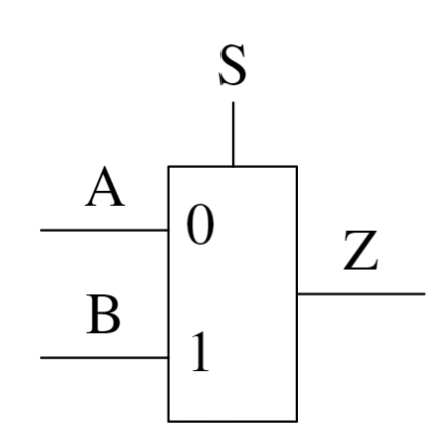
\includegraphics[width= 100px]{images/multiplexer.png}
\end{center}
It outputs A when S is 0, and B when S is 1. It allows us to select between different functions, such as adding and subtracting.\\
Truth tables are another form of representation of a digital system. We will later learn how to analyze and derive equations from truth tables, as well as the gate implementation.\\
\textit{Note: CMOS logic doesn't have AND, OR gates, so the actual implementation of these two is NAND, NOR gates with an inverter.}\\
Gates require 4 transistors, and inverters need two transistors.
Verilog Structural model:
\begin{lstlisting}
    module Ch1mux_s(A,B,S,Z);
        input A,B,S;
        output Z;
        wire SN,ASN,SB;
        not U1(SN,S);
        and U2(ASN,A,SN);
        and U3(SB,B,S);
        or U4(Z,ASN,SB);
    endmodule
\end{lstlisting}
Which is equivalent to:
\begin{center}
    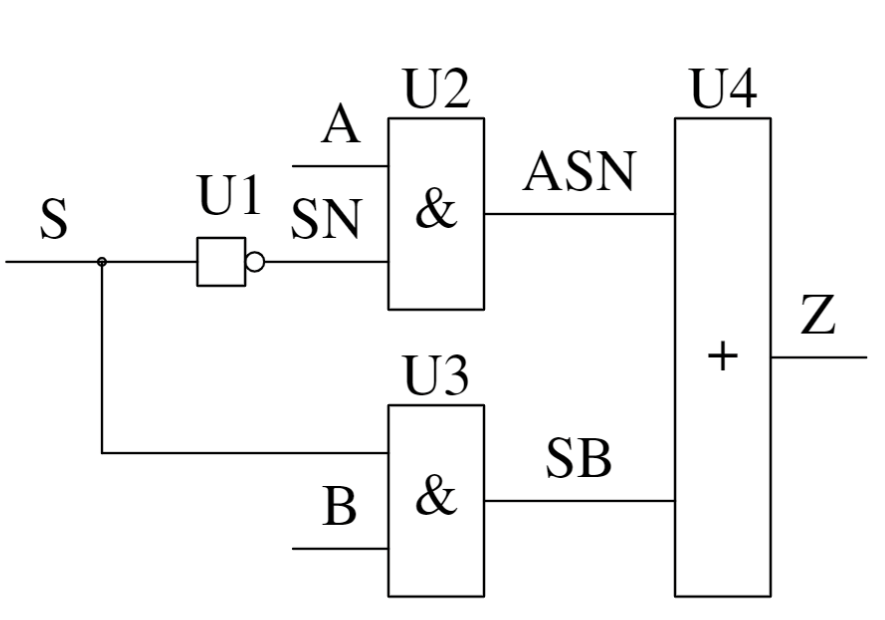
\includegraphics[width= 150px]{images/verilog_implementation.png}
\end{center}
\textit{Note: the order of these statements is irrelevant, they will result in the same digital system.}
Verilog Behavioral Model:
\begin{lstlisting}
    module Ch1mux_b(A,B,S,Z);
        input A,B,S; \\input declaration
        output reg Z; \\output declaration
        always @(A,B,S) \\if input changes, recompute
        if (S==1) Z=B; 
        else Z=A; \\this is saying what the multiplexer above did
    endmodule
\end{lstlisting}
\section{Number Systems and Codes}
A digital circuit processes binary digits in the form of bits.\\ It is
impoortant to see how these relate to real life values.\\ Numbers in the
decimal system:
\begin{equation*}
    abcd = 1000a+100b+10c+d = 10^3a+10^2b+10^1c+10^0d
\end{equation*}
The base, or radix is 10.
For a general radix $r$, it would be:
\begin{equation*}
    abcd = r^3a+r^2b+r^1c+r^0d
\end{equation*}
For this course, we care about binary, or radix 2.\\
Occasionally, base 8 (octal) and base 16 (hexadecimal) are also relevant.
\begin{table}
    \centering
    \begin{tabular}{c|c|c}
        base 2 & base 8 & base 16 \\
        \hline
        0      & 0      & 0       \\
        1      & 1      & 1       \\
        10     & 2      & 2       \\
        11     & 3      & 3       \\
        100    & 4      & 4       \\
        101    & 5      & 5       \\
        110    & 6      & 6       \\
        111    & 7      & 7       \\
        1000   & 10     & 8       \\
        1001   & 11     & 9       \\
        1010   & 12     & A       \\
        1011   & 13     & B       \\
        1100   & 14     & C       \\
        1101   & 15     & D       \\
        1110   & 16     & E       \\
        1111   & 17     & F       \\
    \end{tabular}
\end{table}
To convert from octal to binary, replace every octal with three bits starting from the least significant bit.  For hexadecimal, replace each digit with 4 bits.\\
The least significant bit(LSB) is the last bit, and the first is the most significant bit (MSB).\\
To convert from decimal to binary by dividing the number by 2, and assigning the remainder to the least siginificant unassigned bit. Do this continuously to the quotient until done.\\
\subsection{Adding and Subtracting}
To add and subtract in binary:\\
\begin{table}
    \centering
    \begin{tabular}{c c c c c c}
          & 1 & 0 & 1 & 1 & + \\
          & 1 & 0 & 1 & 0 &   \\
        \hline
        1 & 0 & 1 & 0 & 1
    \end{tabular}
    \quad\quad
    \begin{tabular}{c c c c c c}
        1 & 1 & 0 & 1 & 1 & - \\
          & 1 & 0 & 1 & 0 &   \\
        \hline
        1 & 0 & 0 & 0 & 1 &
    \end{tabular}
\end{table}
To add signs to numbers, it has been standardized that the first bit defines the sign. If the leftmost bit is 0, the number is posititve. and if it is 1, the number is negative. \\This allows an n-bit signed integer to be from the range $-2^{n-1}+1 \text{ to } 2^{n-1}-1.$\\
To actually add and subtract numbers, we first check if the sign is the same, if it is, we add directly, and append the sign bit. If they have opposing signs, we find the larger number, subtract the smaller, and use the sign of the larger.\\
\subsection{Using the complement to conduct operations}
In the complement number system, we can add or subtract directly, the
operations can be done directly. The complementation process is more
complicated than sign checking, but it simplifies addition.\\ The 2-complement
system is the difference between $2^n$ and the n-bit integer. To compute $-B$,
we first need to calculate $2^n-B$, which we can compute as $(2^n-1)-B+1$,
which is essentially inverting each bit, and adding 1 to the result. (Carries
outside the bit length are ignored.)\\ The most significant bit of the
complement acts as a sign bit. This can be seen in the following table:
\begin{table}
    \centering
    \begin{tabular}{c c|c c}
        number & binary & negative & binary \\
        \hline
        0      & 0000   & -0       & 0000   \\
        1      & 0001   & -1       & 1111   \\
        2      & 0010   & -2       & 1110   \\
        3      & 0011   & -3       & 1101   \\
        4      & 0100   & -4       & 1100   \\
        5      & 0101   & -5       & 1011   \\
        6      & 0110   & -6       & 1010   \\
        7      & 0111   & -7       & 1001   \\
        -      & -      & -8       & 1000   \\

    \end{tabular}
\end{table}
The magnitude of a number can be computed as for an unsigned number, except that the weight of the MSB is $-2^{n-1}$ instead of $2^{n-1}$. So, to subtract $2^n$, replace the weight of the MSB with $-2^{n-1}$.\\
To add a bit to a complement number, we can simply duplicate the MSB at the beginning of the MSB.
As proof of this actually working, we can calculate the complement of both the complement and the modified complement as uncomplemented numbers, and we can observe that they will be the same.\\
That is, the complement of 11001 and 111001 is the same number, the same happens for 011 and 0011.\\
We can also reverse this process if the digits corresponding to the removed bits of the given complement are all the same.\\
Now we will analyze how the complement can be used to add and subtract.\\
\begin{center}
    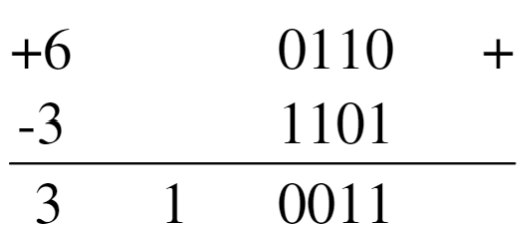
\includegraphics[width = 100px]{images/add_complement.png}
\end{center}
This process may not work if overflow occurs. That is, if the number of necessary bits to represent the result of an operation are more than the available bits. This can only occur if the numbers being operated on have the same sign.\\
To subtract two numbers, we instead use the following property: $X-Y = X+(-Y) = X+Y'+1$ where $Y'$ is the complement of $Y$.
\begin{center}
    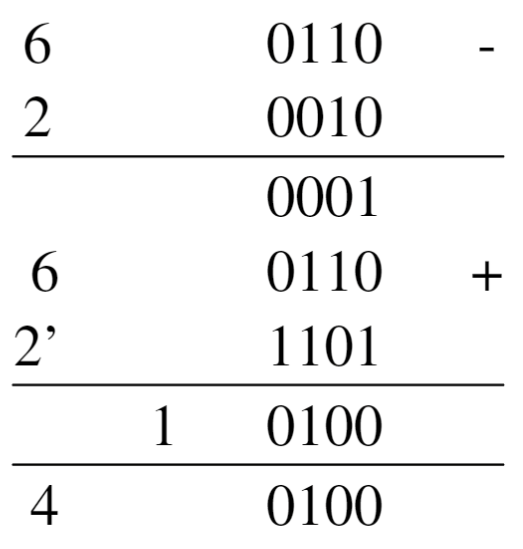
\includegraphics[width = 100px]{images/complement_subtraction.png}
\end{center}
\subsection{Binary Codes for Decimal Numbers}
A set of \textit{n}-bit strings in which differnt bit strings represent
diffferent elements of a set is called a code. A combination on these is a code
word.\\ 0 through 9 requires at least 4 bits, but there are many methods of
doing so.\\
\begin{center}
    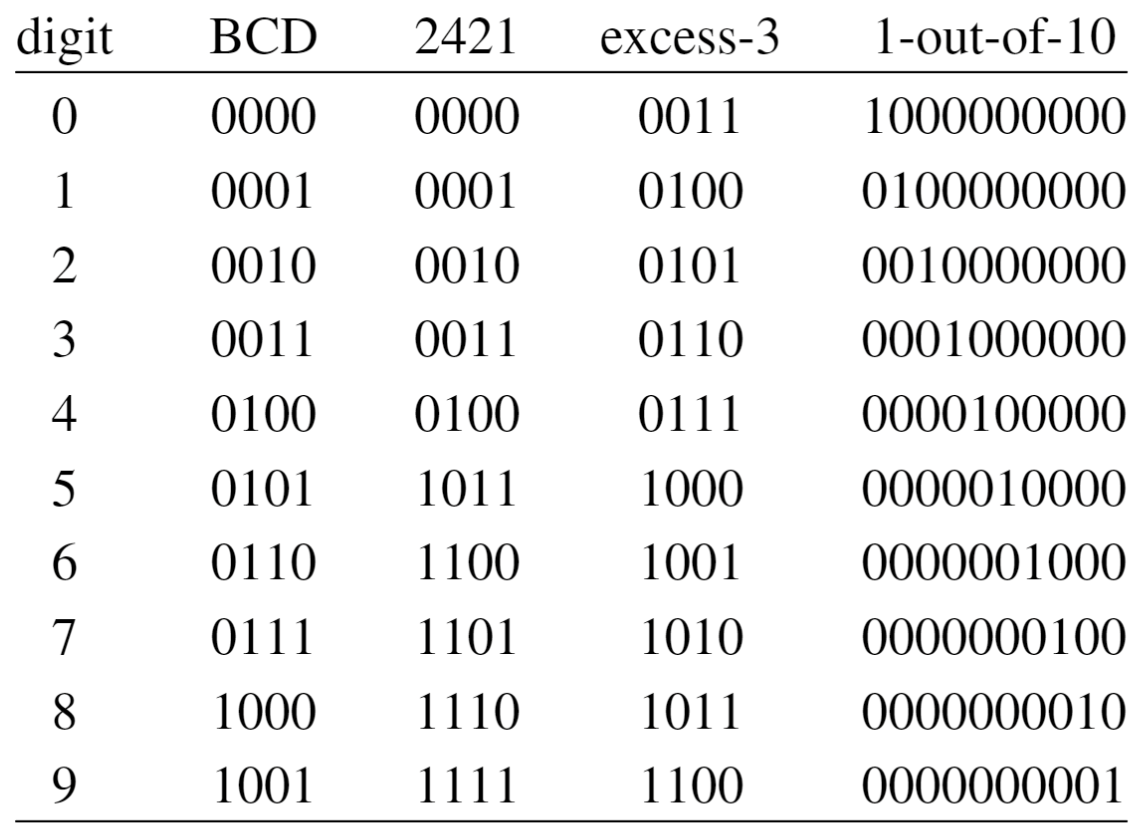
\includegraphics[width = \textwidth]{images/decimal_codes.png}
\end{center}
Another very important representation is the gray code.\\
By partitioning a disk into eight regions, with n bits with sensors in each, any number between 0 and $2^n -1$ can be represented.\\
\begin{center}
    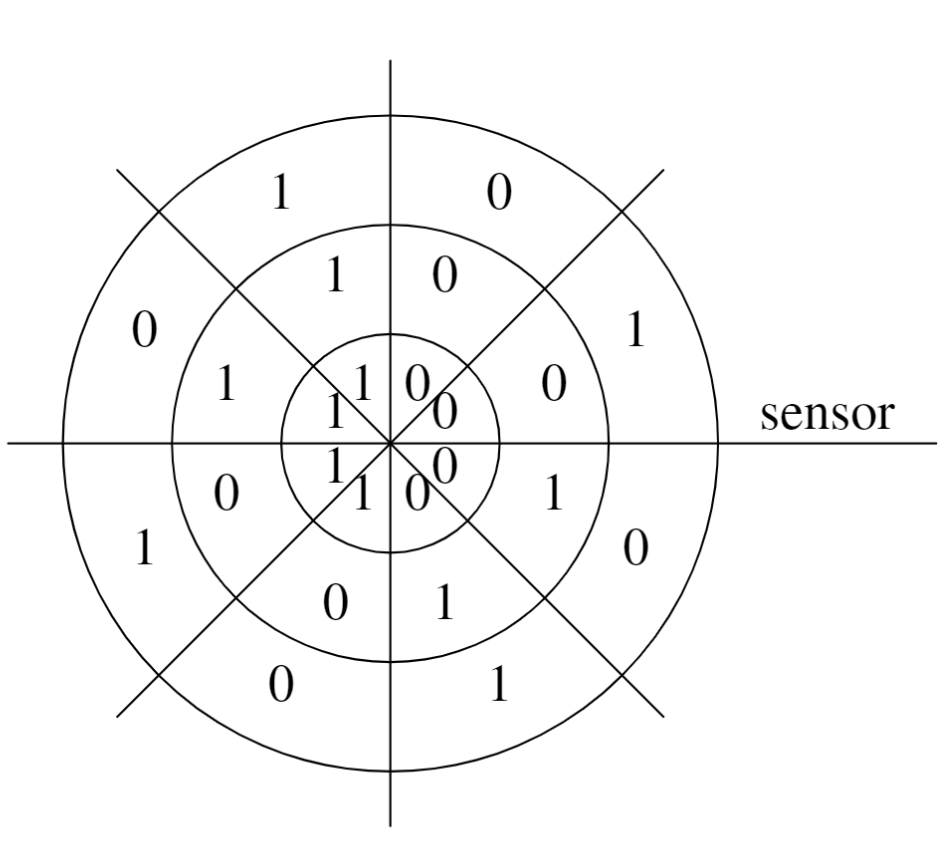
\includegraphics[width = 200px]{images/gray_code.png}
\end{center}
\textit{Note: if the disk stops between two sections, there is a possibility of error. Using standard binary representation will cause the error to be very large, as it can stop between 000 and 111, which would imply that any of the bits can have error, and thus any of the numbers between 0 and 7 can be represented.}
This is where the gray code comes in:\\
\begin{table}
    \centering
    \begin{tabular}{c|c}
        number & gray code \\
        \hline
        0      & 000       \\
        1      & 001       \\
        2      & 011       \\
        3      & 010       \\
        4      & 110       \\
        5      & 111       \\
        6      & 101       \\
        7      & 100       \\
    \end{tabular}
\end{table}
This encoding allows there to be only one bit of change between any two consecutive digits, allowing us to reduce the margin of error.\\
Codes can also be used to represent text, as the ASCII does, which uses a 7-bit code word.\\
The selection of code and code words is very important, as it can drastically change the complexity of the designed circuit:
\begin{center}
    \centering
    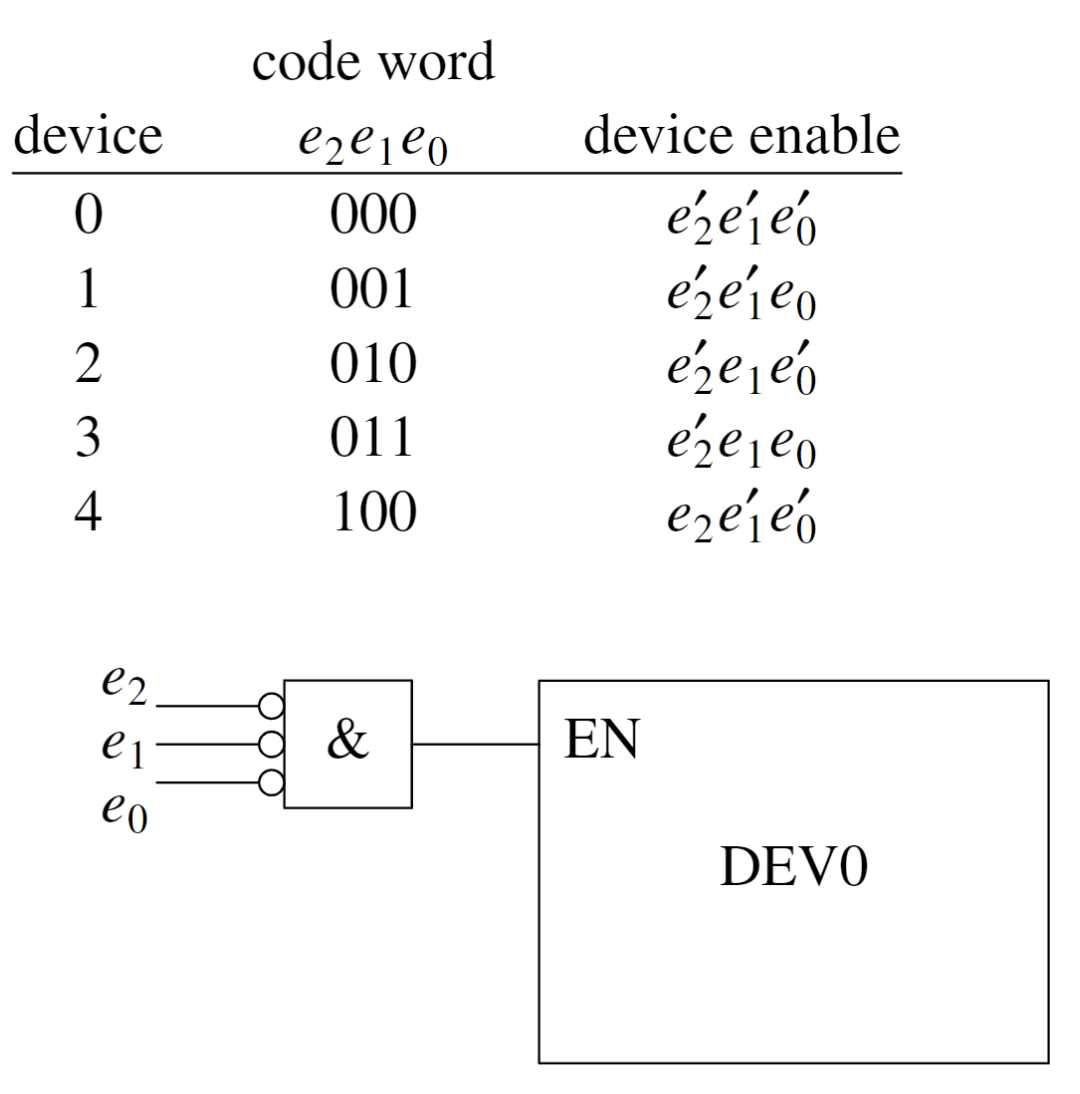
\includegraphics[width = 100px]{images/code_ex1.png} \quad
    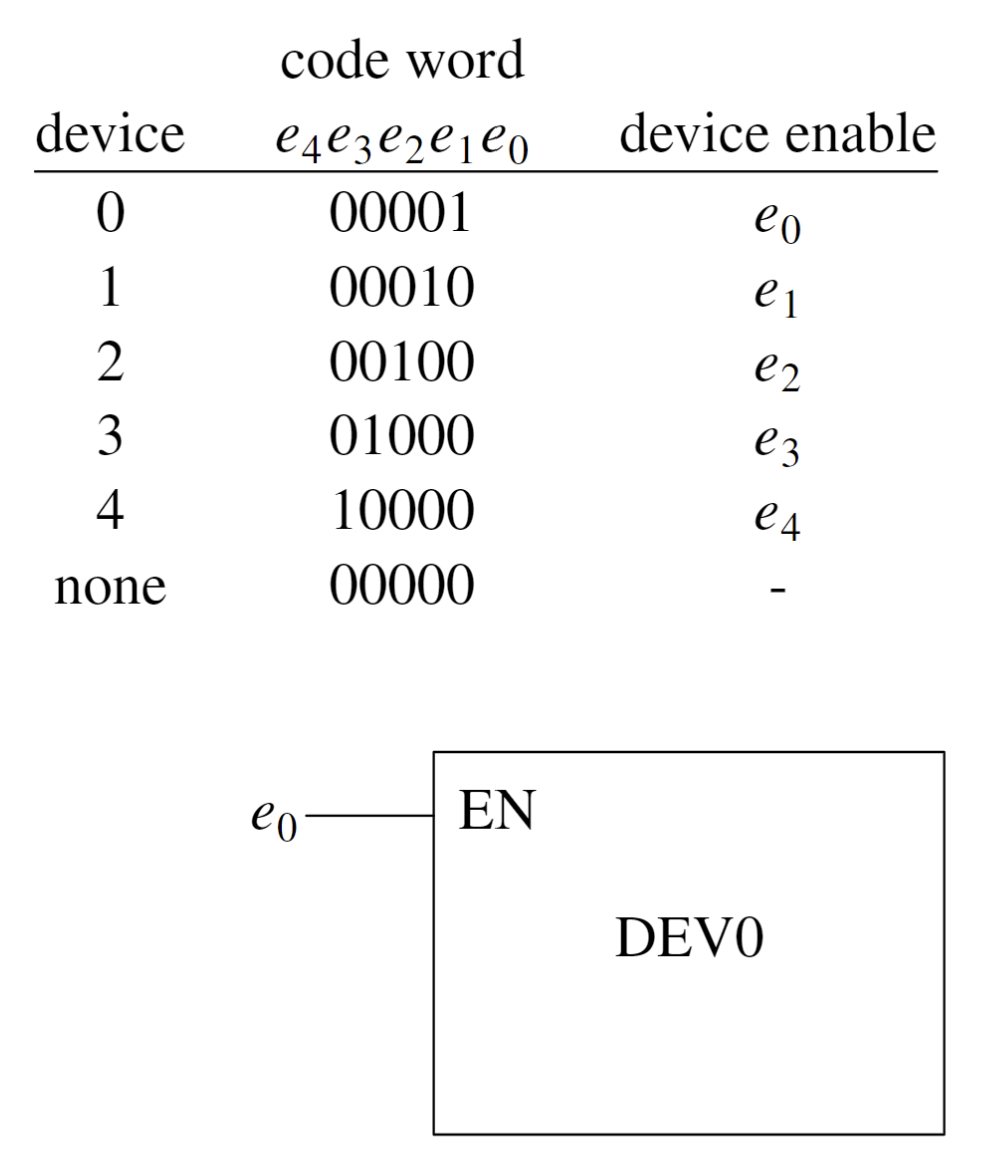
\includegraphics[width = 100px]{images/code_ex2.png}
\end{center}
\section{Switching Algebra and Combinational Logic}
A combinational circuit depends only on the inputs. We will begin by
considering single ouptut combinational circuits.\\ Switching algebra is a
mathematical tool used for circuit design. It is a subset of boolean algebra. A
variable is used to represent a signal.\\
\subsection{Axioms}
\begin{itemize}
    \item (A1) $X=0$ if $X \neq 1$
    \item (A1D) $X=1$ if $X \neq 0$
\end{itemize}
There is a principle of duality in this axiom, as do most properties of switching algebra.\\
\begin{itemize}
    \item (A2) $X=0 \implies X' = 1$
    \item (A2D) $X=1 \implies X'=0$
    \item (A3) $0 \land 0 = 0$
    \item (A4) $1 \land 1 = 1$
    \item (A5) $0\land 1 = 1\land 0 = 0$
    \item (A6) $ 1 \lor 1=1$
    \item (A7) $0\lor 0 = 0$
    \item (A8) $1\lor 0 = 0\lor 1 = 1$
\end{itemize}
AND has a higher precedence than OR in logical expressions"
\begin{equation*}
    W\land Y \lor Y\land Z = (W\land X) \lor (Y\land Z)
\end{equation*}
There are 5 theorems that can be easily be proven through this:
\begin{enumerate}
    \item $X\lor 0=X$
    \item $X \lor 1 = 1$
    \item $X \lor X = X$
    \item $(X')'=X$
    \item $X\lor X' = 1$
\end{enumerate}
Which have the following dualities:
\begin{enumerate}
    \item $X\land 1 =X$
    \item $X\land 0 = 0$
    \item $X \land X = X$
    \item No duality
    \item $X\land X' = 0$
\end{enumerate}
There are also two variable theorems:
\begin{itemize}
    \item Commutativity:
    \begin{enumerate}
        \item $X\lor Y=Y\lor X$
        \item $X\land Y = Y\land X$
    \end{enumerate}
    \item Associativity: \begin{enumerate}
        \item $(X\lor Y)\lor Z=X\lor (Y\lor Z)$
        \item $(X\land Y)\land Z=X\land (Y\land Z)$
    \end{enumerate}
    This allows for the representation of three or more input gates with ease.
\end{itemize}
\end{document}